% Drawing 29/06-2 -- folder 29, batch 06, archive page 106 (PDF page 107).
% Transcription: en haut de la page, un dessin : deux branches, $X_{T'}$ horizontale et $X_{T''}$ verticale, se coupant en un point ; de part et d'autre du point, chaque branche est doublée d'un faisceau de deux traits qui s'évasent en s'éloignant, hachuré de petits traits transverses ; autour du point de croisement, un disque semé de points porte la lettre $Z$.
% Kind: two branches X_T' and X_T'' crossing at a point, with a dotted disc Z. Method 2 (schematic redraw from the facsimile). Status: ok.
% Notes: The horizontal line X_T' (ending at the right in a short downward hook) and the vertical line X_T'' through one crossing point (the vertical above the crossing is a faint pencil guide; below it the line is heavy); on each of the four half-branches a wedge of two curved strokes opening away from the crossing point (drawn from that point), hatched with short transverse strokes as on the page: four oblique ones above (rising to the right), four below (three across the wedge and a short one from the line to the right stroke), three on the left and a faint fourth (pencil), four on the right; the disc round the crossing point, open at the lower left (the outline is a full line, not dotted, against the note of the transcription), with seventeen dots inside it and the letter Z in its upper right part; the labels X_T'' (top) and X_T' (right). Overlaid 2026-11-12 (Opus 5.5) on the 400 dpi colour crop and redrawn: the wedges were straight and their hatches horizontal across the upper and lower ones; the disc was a circle 1 unit too small at the right and closed; the line X_T' ran 20 units short of its end (to 100.5) and the end of its pencil continuation was not on the page. Redrawn 2026-11-12 (issue 128): to check again.
% Coordinates: 1 unit = 0.8 mm = 1/100 of the crop width (bbox in page fractions: [0.15, 0.13, 0.55, 0.32]).
% Redrawn by Claude (claude-fable-5-2), issue #128, 2026-11-12; not checked by a human; not compiled (no TeX in the session).
% Overlaid by Claude (claude-opus-5-5) 2026-11-12 (issue #128): rasterised from its own coordinates over the 400 dpi colour facsimile and corrected from it. Not compiled. Status: ok.
% Rights: reproduces part of the work -- behind RENDER_TRANSCRIPTS, never published by itself.
\documentclass[tikz,border=3pt]{standalone}
\usepackage{amsmath,amssymb}
\usetikzlibrary{patterns,arrows.meta}
\tikzset{pencil/.style={black!45}, struck/.style={black!35}, mpt/.style={circle,draw,inner sep=1.3pt}, pt/.style={circle,fill,inner sep=0.9pt}, opt/.style={circle,draw,fill=white,inner sep=1.1pt}}
\begin{document}
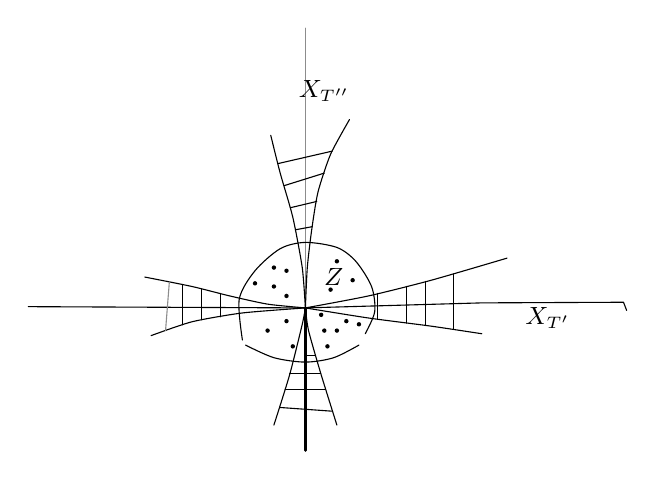
\begin{tikzpicture}[x=0.8mm,y=0.8mm,line cap=round,line join=round,font=\scriptsize]
\draw (6,-44.2) -- (50,-44.4) -- (78,-43.6) -- (100.5,-43.5) -- (101,-44.8);
\draw[pencil] (50,0) -- (50,-44.4);
\draw[very thick] (50,-44.4) -- (50,-67);
\draw plot[smooth, tension=0.4] coordinates {(44.5,-17) (46,-23) (48,-30) (49.5,-38) (50,-44.4)};
\draw plot[smooth, tension=0.4] coordinates {(57,-14.5) (54,-20) (52,-26) (51,-32) (50.3,-38) (50,-44.4)};
\draw plot[smooth, tension=0.4] coordinates {(50,-44.4) (49.5,-47) (47.5,-55) (45,-63)};
\draw plot[smooth, tension=0.4] coordinates {(50,-44.4) (50.5,-48) (52.5,-55) (55,-63)};
\draw plot[smooth, tension=0.4] coordinates {(24.5,-39.5) (32,-41) (38,-42.5) (44,-43.8) (50,-44.4)};
\draw plot[smooth, tension=0.4] coordinates {(25.5,-48.8) (32,-46.6) (40,-45.2) (50,-44.4)};
\draw plot[smooth, tension=0.4] coordinates {(50,-44.4) (60,-42.5) (70,-40) (82,-36.5)};
\draw plot[smooth, tension=0.4] coordinates {(50,-44.4) (60,-46) (70,-47.3) (78,-48.5)};
\draw (45.6,-21.5) -- (54.3,-19.5);
\draw (46.6,-25.0) -- (53.0,-23.0);
\draw (47.6,-28.5) -- (51.8,-27.5);
\draw (48.4,-32.0) -- (51.1,-31.5);
\draw (47.5,-54.8) -- (52.4,-54.8);
\draw (46.8,-57.3) -- (53.2,-57.3);
\draw (45.9,-60.2) -- (54.3,-60.8);
\draw (50,-52) -- (51.6,-52.0);
\draw (30.5,-40.7) -- (30.5,-47.1);
\draw (33.5,-41.4) -- (33.5,-46.3);
\draw (36.5,-42.1) -- (36.5,-45.8);
\draw[pencil] (28.4,-40.3) -- (27.8,-48.0);
\draw (61.5,-42.1) -- (61.5,-46.2);
\draw (66.0,-41.0) -- (66.0,-46.8);
\draw (69.0,-40.2) -- (69.0,-47.2);
\draw (73.5,-39.0) -- (73.5,-47.8);
\draw plot[smooth, tension=0.5] coordinates {(40,-49.5) (39.5,-43) (42,-38.5) (46,-35) (50,-34) (55,-34.8) (58,-37) (60.5,-41) (61,-45) (59.5,-48.5)};
\draw plot[smooth, tension=0.5] coordinates {(40.5,-50.3) (45,-52.3) (50,-53) (54.5,-52.3) (58.5,-50.3)};
\fill (45,-38) circle[radius=0.35];
\fill (47,-38.5) circle[radius=0.35];
\fill (42,-40.5) circle[radius=0.35];
\fill (45,-41) circle[radius=0.35];
\fill (47,-42.5) circle[radius=0.35];
\fill (55,-37) circle[radius=0.35];
\fill (57.5,-40) circle[radius=0.35];
\fill (54,-41.5) circle[radius=0.35];
\fill (52.5,-45.5) circle[radius=0.35];
\fill (47,-46.5) circle[radius=0.35];
\fill (44,-48) circle[radius=0.35];
\fill (48,-50.5) circle[radius=0.35];
\fill (53,-48) circle[radius=0.35];
\fill (55,-48) circle[radius=0.35];
\fill (56.5,-46.5) circle[radius=0.35];
\fill (58.5,-47) circle[radius=0.35];
\fill (53.5,-50.5) circle[radius=0.35];
\node[inner sep=1pt] at (54.5,-39.5) {\small $Z$};
\node[inner sep=1pt] at (53,-10) {\small $X_{T''}$};
\node[inner sep=1pt] at (88.5,-46) {\small $X_{T'}$};
\end{tikzpicture}
\end{document}
